% ------------------------- REVISADO
\mychapter{Metodologia}
\label{Cap:Metodologia}

Este capítulo aborda a metodologia aplicada no desenvolvimento do \textit{software} RADARE, detalhando os métodos de engenharia de \textit{software} utilizados durante o processo, desde a concepção até a prototipação. São explorados o projeto geral do desenvolvimento do RADARE, a arquitetura do sistema, o versionamento adotado, o ambiente de desenvolvimento e as linguagens escolhidas. As subseções incluem o uso do TypeScript no desenvolvimento do \textit{front-end}, do Python no desenvolvimento do \textit{back-end} e do PostgreSQL como banco de dados. Cada uma dessas áreas é discutida com foco na contribuição para a funcionalidade e eficiência do \textit{software}.

% ------------------------- REVISADO
\section{Projeto de desenvolvimento do RADARE}

Uma metodologia de desenvolvimento de \textit{software} é um conjunto de práticas que guia o processo de criação de sistemas, organizando etapas como análise, design, implementação e teste. Ela otimiza a produtividade e a qualidade, ajudando a gerenciar recursos e prazos. A escolha da metodologia depende das necessidades do projeto e dos objetivos do \textit{software}.

% ------------------------- REVISADO
\subsection{Metodologia de desenvolvimento do \textit{software}}

O desenvolvimento do \textit{software} RADARE adotou o método ágil Scrum, escolhido por sua adequação ao desenvolvimento iterativo e adaptável com um único desenvolvedor \cite{softwareengreq}. Com o Scrum, o projeto foi organizado em \textit{sprints} de duração definida, onde o trabalho foi focado em metas prioritárias, facilitando ajustes rápidos conforme surgiam novas necessidades.

O Scrum permitiu uma gestão eficiente com revisões periódicas e reuniões de monitoramento, onde eram avaliados o progresso e as próximas ações. As revisões de \textit{sprint} possibilitaram validações frequentes e garantiram que as funcionalidades desenvolvidas estivessem alinhadas com os objetivos do RADARE. 

Ao longo do projeto, o Scrum viabilizou uma abordagem flexível e produtiva, otimizando a entrega de valor e adaptando-se rapidamente às demandas do desenvolvimento do \textit{software}.

% ------------------------- REVISADO
\subsection{Escopo do \textit{software}}

O escopo do projeto define os limites do trabalho a ser realizado, garantindo que todas as atividades estejam alinhadas com os objetivos do projeto. Isso proporciona uma base sólida para o planejamento, execução e controle do desenvolvimento do \textit{software}, permitindo a concentração nas entregas essenciais para o projeto \cite{softwareeng}.

% ------------------------- REVISADO
\subsection{Requisitos funcionais do sistema}

Os requisitos funcionais no projeto de \textit{software} desempenham um papel crucial na definição das capacidades e funcionalidades que o sistema deve fornecer para atender às necessidades dos usuários. Em suma, eles representam o "o que" o sistema deve fazer. Esses requisitos são geralmente expressos em termos de casos de uso, cenários de interação do usuário ou fluxos de trabalho \cite{softwareengreq}.
        
A Tabela \ref{tab:req_funcional} demonstra os atuais requisitos funcionais do \textit{software}.

\begin{table}[htbp]
\centering
\begin{tabularx}{\linewidth}{|c|X|c|c|} \hline
\rowcolor[HTML]{C0C0C0} 
\textbf{Identificador} & \textbf{Descrição} & \textbf{Prioridade} & \textbf{Requisitos Relacionados} \\ \hline
RF01 & O sistema deve permitir que os usuários modelem a dinâmica dos sensores em uma planta industrial. & Alta & RF02 \\ \hline
RF02 & Os usuários devem ser capazes de alimentar o sistema com os dados gerados pelos sensores. & Alta & RF01 \\ \hline
RF03 & O sistema deve oferecer um painel para visualização em tempo real dos dados reconciliados. & Média & RF01, RF02 \\ \hline
RF04 & O sistema deve ser capaz de entregar a reconciliação de dados de forma rápida e correta. & Alta & RF01 \\ \hline
RF05 & Os usuários devem poder exportar os dados reconciliados para diferentes formatos de arquivo. & Média & RF03 \\ \hline
\end{tabularx}

\caption{Tabela modelo dos requisitos funcionais.}
\label{tab:req_funcional}
\end{table}

% ------------------------- REVISADO
\subsection{Requisitos não funcionais do sistema}

Os requisitos não funcionais em um projeto de \textit{software} desempenham um papel igualmente crucial, complementando os requisitos funcionais ao definir os critérios de qualidade, desempenho e restrições operacionais que o sistema deve atender. Enquanto os requisitos funcionais se concentram no "o que" o sistema deve fazer, os requisitos não funcionais delineiam "como" o sistema deve fazer isso, bem como outras características importantes que afetam sua operação e usabilidade e muitas vezes abordam características mais abstratas do sistema, como segurança, confiabilidade, escalabilidade, desempenho e usabilidade \cite{softwareengreq}. 
            
A Tabela \ref{tab:ReqNaoFuncional} demonstra os atuais requisitos não funcionais do \textit{software}.

\begin{table}[htbp]
\centering
\begin{tabularx}{\linewidth}{|c|X|c|c|} \hline
\rowcolor[HTML]{C0C0C0} 
    \textbf{Identificador} & \textbf{Descrição} & \textbf{Prioridade} \\
    \hline
    RNF01 & O sistema deve ser altamente escalável para lidar com um grande volume de dados. & Alta \\
    \hline
    RNF02 & A segurança dos dados deve ser uma prioridade, garantindo proteção contra acesso não autorizado e manipulação indevida. & Alta \\
    \hline
    RNF03 & O desempenho do sistema deve ser otimizado para garantir tempos de resposta rápidos, mesmo em momentos de pico de uso. & Alta \\
    \hline
    RNF04 & O sistema deve ser facilmente configurável e customizável para atender às necessidades específicas de diferentes ambientes industriais. & Média \\
    \hline
    RNF05 & A manutenibilidade do sistema deve ser uma consideração fundamental, facilitando atualizações, correções de bugs e modificações futuras. & Média \\
    \hline
    RNF06 & A usabilidade do sistema deve ser intuitiva, permitindo uma curva de aprendizado mínima para os usuários. & Média \\
    \hline
    RNF07 & O sistema deve ser compatível com diferentes navegadores, garantindo sua acessibilidade em uma variedade de ambientes de implantação. & Alta \\
    \hline
    RNF08 & O sistema deve estar em conformidade com regulamentações de privacidade de dados, como GDPR, garantindo o tratamento adequado e a proteção das informações pessoais dos usuários. & Alta \\
    \hline
    RNF09 & A tolerância a falhas do sistema deve ser implementada, garantindo a continuidade das operações mesmo em caso de falhas de componentes individuais. & Alta \\
    \hline
    RNF10 & O tempo de resposta do sistema deve ser consistente e previsível, independentemente da carga de trabalho ou do número de usuários simultâneos. & Média \\
    \hline
\end{tabularx}
\caption{Tabela de Requisitos Não Funcionais}
\label{tab:ReqNaoFuncional}
\end{table}

% ------------------------- REVISADO
\subsection{Temporização do desenvolvimento do \textit{software}}

O Gráfico de Gantt é uma ferramenta essencial no gerenciamento de projetos, permitindo visualizar e acompanhar o progresso das atividades ao longo do tempo. Desenvolvido por Henry Gantt na década de 1910, o gráfico organiza as tarefas em barras horizontais ao longo de um eixo de tempo, facilitando a identificação das datas de início e término, além das interdependências entre atividades \cite{ganttchart}.

\begin{figure}[h]
    \centering
    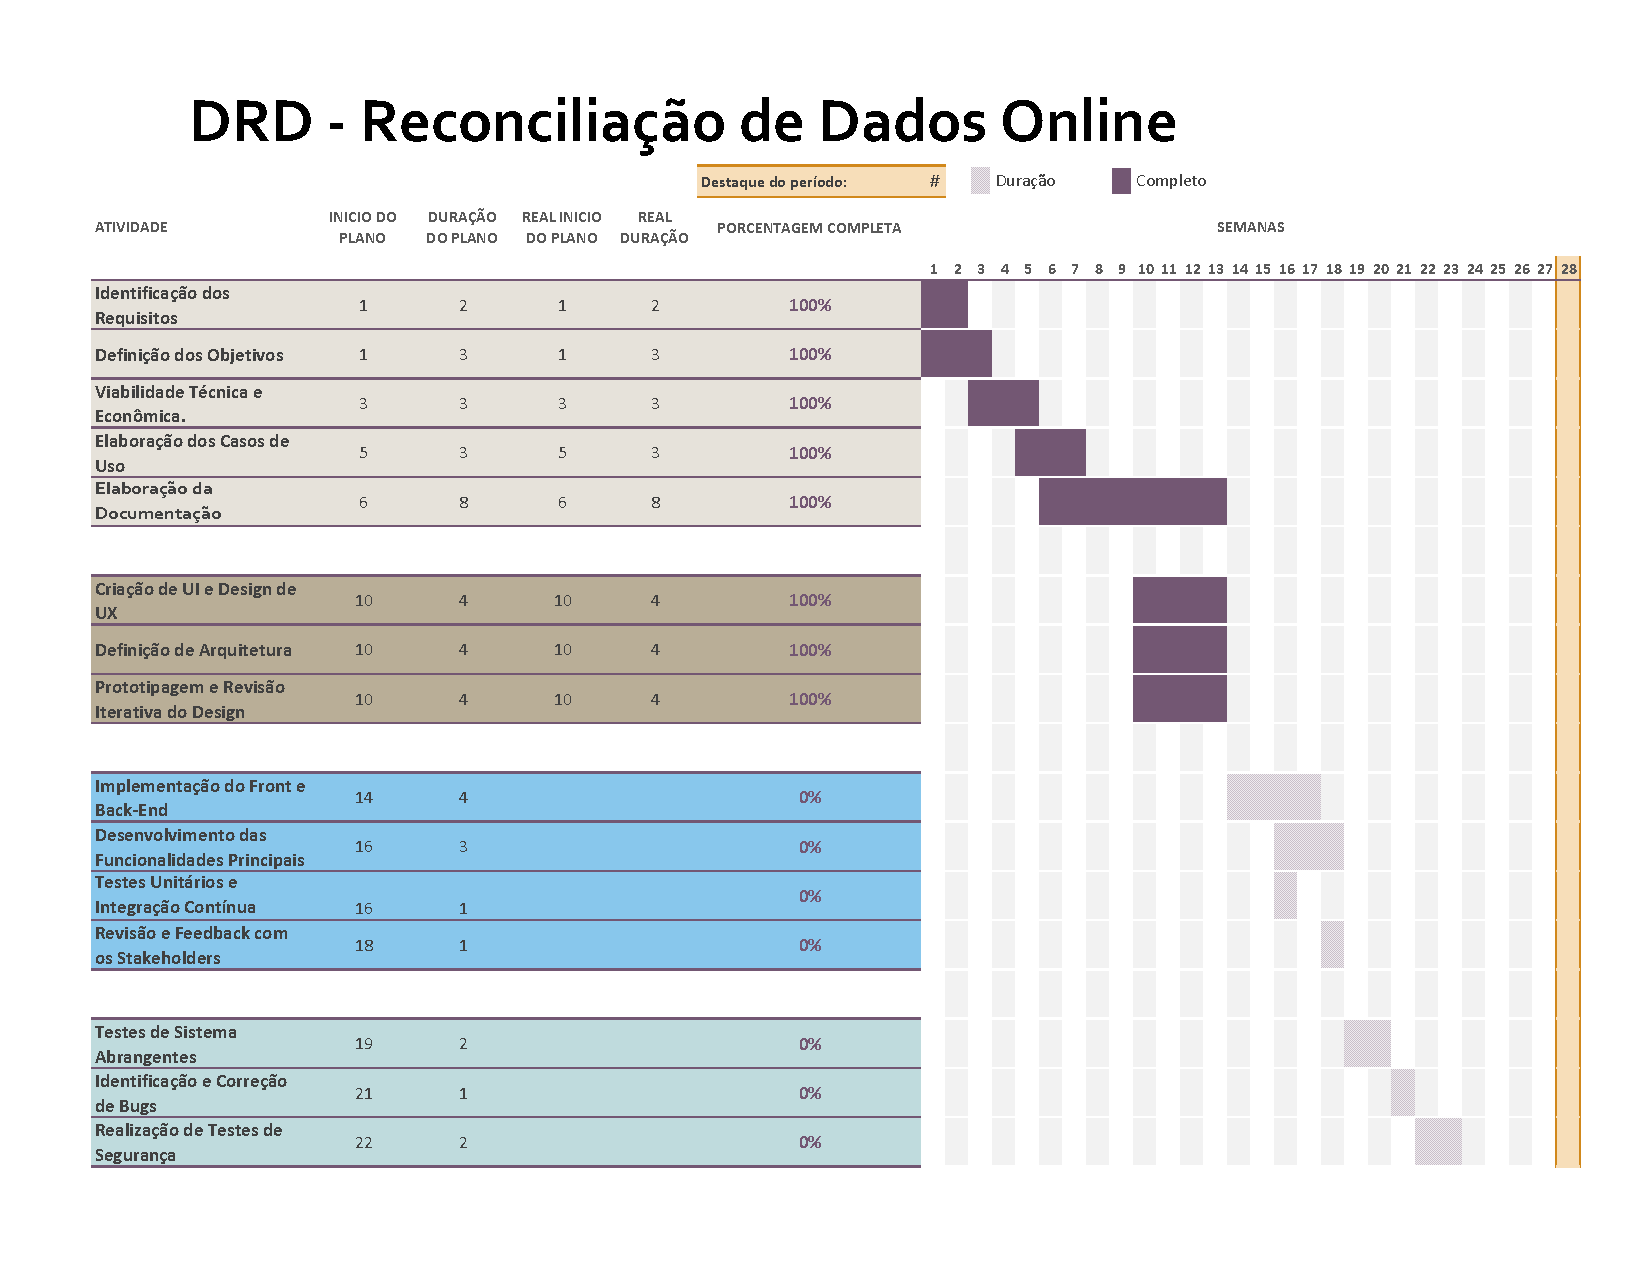
\includegraphics[width=0.8\textwidth]{figuras/DRD-Ganttt.pdf} % Replace "example.pdf" with the path to your PDF file
    \caption{Grafico de Gantt para desenvolvimento do \textit{software} RADARE.}
    \label{fig:ganttChart}
\end{figure}    

Na Figura \ref{fig:ganttChart} é visível Gráfico de Gantt utilizado pelo projeto, onde ele é separado nas seguintes partes: 
    
\begin{itemize}
    \item \textbf{Planejamento e Análise Inicial:} Esta fase inclui a identificação dos requisitos, definição dos objetivos, análise de viabilidade técnica e econômica, além da elaboração dos casos de uso e da documentação.
    
    \item \textbf{\textit{Design} e Prototipagem:} Nesta etapa, são criados o design de interface do usuário (UI) e o design de experiência do usuário (UX), bem como a definição da arquitetura do sistema e a prototipagem com revisões iterativas do design.
    
    \item \textbf{Desenvolvimento e Implementação:} Aqui ocorre a implementação do \textit{front} e \textit{back-end}, o desenvolvimento das funcionalidades principais do sistema, os testes unitários e a integração contínua, além da revisão e \textit{feedback} com os \textit{stakeholders}.
    
    \item \textbf{Testes e Garantia de Qualidade:} Esta fase abrange os testes de sistema abrangentes, a identificação e correção de \textit{bugs}, e a realização de testes de segurança para garantir a qualidade do sistema.
    
    \item \textbf{Preparação para Lançamento:} Envolve a preparação do ambiente de produção, o treinamento de usuários finais e o lançamento suave do sistema para garantir uma transição tranquila para os usuários.
    
    \item \textbf{Suporte e Manutenção Pós-Lançamento:} Por fim, inclui o monitoramento contínuo do sistema, atualizações regulares de \textit{software} e fornecimento de suporte técnico aos usuários para garantir o bom funcionamento e a satisfação contínua dos clientes.
\end{itemize}

A utilização do gráfico de Gantt foi essencial para organizar temporalmente a produção, auxiliando no planejamento e coordenação das etapas do projeto. Ele permitiu uma rápida avaliação do progresso, destacando visualmente atividades concluídas, em andamento e pendentes, além de identificar áreas de atraso ou gargalos, facilitando a tomada de ações corretivas para manter o projeto no rumo certo.
        
% ------------------------- REVISADO
\section{Arquitetura geral do sistema}

Durante o desenvolvimento de \textit{software}, o uso de representações visuais é fundamental para proporcionar uma compreensão clara das funcionalidades e da estrutura do projeto. A linguagem de modelagem unificada (UML) oferece diversos tipos de diagramas para representar diferentes aspectos do sistema. Para este projeto, foi utilizado o PlantUML \cite{plantumldoc}, que permite a modelagem dos processos por meio de código, facilitando a modificação e atualização dos diagramas \cite{softwareengreq}.

% ------------------------- REVISADO
\subsubsection{Diagrama de Classe}

O diagrama de classes representa a estrutura estática do sistema RADARE, descrevendo as classes, seus atributos e métodos \cite{softwareenguml}, como mostrado na Figura \ref{fig:ClassDiagram}.

\begin{figure}[htb]
    \caption{\label{fig:ClassDiagram}Diagrama de Classe em UML do sistema RADARE.}
    \begin{center}
        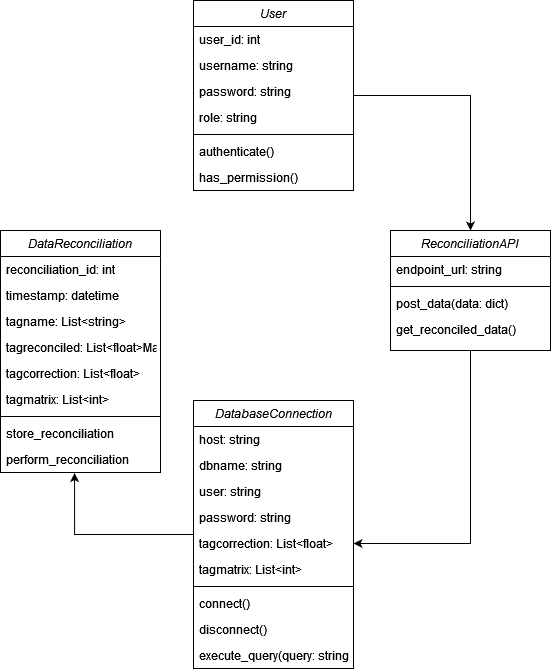
\includegraphics[width=0.6\textwidth]{figuras/ClassDiagramRADARE.drawio.png}
    \end{center}
\end{figure}

Principais classes do sistema:

\begin{itemize}
    \item \textbf{User}: Representa os usuários, com atributos como ID do usuário, nome de usuário, senha e nível de acesso. Inclui métodos de autenticação e verificação de permissões.
    
    \item \textbf{DataReconciliation}: Classe central para cálculos de reconciliação, com atributos como ID da reconciliação, data e hora, variáveis medidas, valores reconciliados e correções aplicadas. Contém o método para executar a reconciliação.
    
    \item \textbf{DatabaseConnection}: Gerencia a conexão com o banco de dados, com métodos para conectar, desconectar e executar consultas.
    
    \item \textbf{ReconciliationAPI}: Interface para comunicação entre \textit{back-end} e \textit{front-end}, com métodos para enviar e recuperar dados reconciliados.
\end{itemize}

Os relacionamentos entre as classes mostram associações e dependências, refletindo as interações entre os componentes do sistema, essenciais para o \textit{design} e análise \cite{softwareenguml}.

% ------------------------- REVISADO
\subsubsection{Diagrama de Caso de Uso}

O diagrama de caso de uso descreve a interação entre o sistema RADARE e seu único usuário, o operador. Ele mostra os principais casos de uso ou funcionalidades do sistema que o operador pode acessar, como ilustrado na Figura \ref{fig:UseCaseDiagram}.

\begin{figure}[htb]
    \caption{\label{fig:UseCaseDiagram}Diagrama de Caso de Uso em UML.}
    \begin{center}
        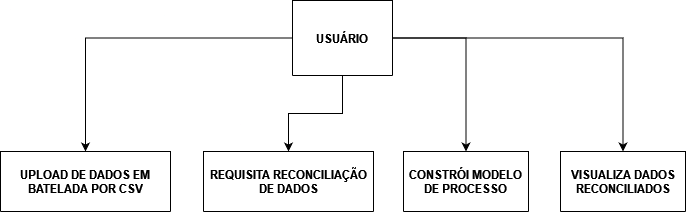
\includegraphics[width=0.6\textwidth]{figuras/DiagramaCasodeUso.drawio.png}
    \end{center}
\end{figure}

Neste diagrama, os casos de uso são:

\begin{itemize}
    \item \textbf{Upload de Dados em Batelada por CSV}: Permite ao usuário carregar arquivos CSV contendo dados de sensores para o sistema.
    \item \textbf{Requisita Reconciliação de Dados}: O usuário solicita a reconciliação dos dados carregados, aplicando o método dos multiplicadores de Lagrange para ajuste de valores.
    \item \textbf{Constrói Modelo de Processo}: Permite ao usuário construir e ajustar o modelo de processo no sistema, configurando os fluxos de dados e pontos de coleta.
    \item \textbf{Visualiza Dados Reconciliados}: Exibe os resultados da reconciliação para que o usuário possa visualizar e analisar os dados ajustados.
\end{itemize}

As conexões entre o ator e os casos de uso representam as interações do usuário com as funcionalidades do sistema.

% ------------------------- REVISADO
\section{Versionamento no desenvolvimento do software}

O desenvolvimento do RADARE utilizou o \textit{Git} (versão 2.46) e o \textit{GitHub} para versionamento e controle de colaboração. O \textit{Git} é um sistema de controle de versão que permite rastrear e gerenciar alterações no código, possibilitando desenvolvimento paralelo e revertendo modificações quando necessário.

\textit{GitHub} hospeda repositórios \textit{Git} na nuvem, facilitando a colaboração entre os membros da equipe. Ferramentas como \textit{pull requests} e \textit{code reviews} foram utilizadas para revisão e validação das alterações antes de integrações ao código principal, garantindo qualidade e consistência.

O uso de \textit{branches} permitiu o desenvolvimento isolado de funcionalidades e correções, com integração ao código principal apenas após validação, facilitando o gerenciamento de versões e minimizando conflitos.


% ------------------------- REVISADO
\section{Ambiente de desenvolvimento do software}

O desenvolvimento do RADARE foi realizado em um ambiente configurado para otimizar a produtividade e a organização dos componentes do sistema. O editor de código \textit{Visual Studio Code (VSCode)} versão 1.78 foi utilizado como ferramenta principal, devido à sua interface intuitiva e suporte a extensões, facilitando a escrita e organização do código. O sistema operacional utilizado foi o \textit{Windows 11} versão 22H2, que ofereceu um ambiente estável e compatível com as ferramentas empregadas no projeto.

Para testar e garantir a compatibilidade do \textit{website}, foram utilizados os navegadores \textit{Microsoft Edge} versão 129, \textit{Google Chrome} versão 130 e \textit{Mozilla Firefox} versão 131. Essa abordagem permitiu avaliar o comportamento e a responsividade da interface em diferentes navegadores, assegurando que o sistema fosse acessível e funcional para uma variedade de usuários.

Informações detalhadas sobre a configuração da máquina utilizada no desenvolvimento do sistema, incluindo especificações de hardware e software, estão disponíveis no \textbf{Apêndice \ref{Ap:configuracaoMaquina}}. Esse ambiente de desenvolvimento foi fundamental para a construção e testes do RADARE, proporcionando as ferramentas necessárias para uma implementação eficiente e controle visual de qualidade.
    
% ------------------------- REVISADO
\section{Linguagem TypeScript no desenvolvimento do front-end}

No desenvolvimento do front-end do RADARE, o TypeScript foi escolhido como a linguagem principal devido à sua tipagem estática opcional, que adiciona estrutura e robustez ao código em comparação ao JavaScript. Com o TypeScript, foi possível definir tipos específicos para variáveis, funções e objetos, reduzindo a ocorrência de erros de tipo e facilitando a detecção de problemas ainda na fase de desenvolvimento. Além disso, o uso de interfaces e classes trouxe uma organização clara dos componentes, promovendo a reutilização de código e facilitando a implementação modular.

A estrutura do projeto foi baseada em uma abordagem modular, onde cada componente foi desenvolvido como uma unidade independente. Isso facilitou a manutenção e a escalabilidade, especialmente para os elementos visuais do \textit{canvas}, onde cada nódulo e conexão pode ser manipulado de forma individual. A tipagem garantiu que todos os elementos do \textit{canvas} tivessem propriedades definidas, como posição e estado, assegurando interações consistentes entre os módulos.

Para a construção da interface visual, o TypeScript foi integrado ao HTML e SCSS, com o HTML definindo a estrutura dos elementos e o SCSS cuidando do design e layout. O TypeScript coordenou as interações entre a interface e a lógica de negócios, tornando a interface responsiva e interativa, reagindo às entradas do usuário de maneira dinâmica.

% ------------------------- REVISADO
\section{Linguagem Python no desenvolvimento do \textit{back-end}}

A linguagem \textit{Python} (versão 3.12) foi escolhida para o desenvolvimento do \textit{back-end} do RADARE devido à sua simplicidade, flexibilidade e à ampla variedade de bibliotecas disponíveis, que facilitam a implementação de funcionalidades essenciais em sistemas de reconciliação de dados. Python é reconhecido pela sua clareza e legibilidade, características que tornam o desenvolvimento mais eficiente e reduzem o tempo necessário para depuração e manutenção do código. Além disso, o suporte robusto a cálculos numéricos e estatísticos através de bibliotecas como \textit{NumPy} e \textit{SciPy} permite realizar operações complexas de maneira otimizada, um aspecto crucial para o processamento de dados em tempo real.

Para a criação de uma API RESTful que facilita a comunicação entre o \textit{front-end} e o banco de dados, foi utilizado o microframework \textit{Flask}. \textit{Flask} é uma ferramenta leve e modular que oferece flexibilidade para a construção de aplicações \textit{web} sem impor uma estrutura rígida. Essa flexibilidade é vantajosa no desenvolvimento do RADARE, pois permite a implementação de \textit{endpoints} customizados para manipulação de dados, que se ajustam facilmente às necessidades específicas do sistema de reconciliação.

Além disso, \textit{Flask} integra-se perfeitamente com \textit{Psycopg2}, uma biblioteca que permite conectar o \textit{Python} ao banco de dados \textit{PostgreSQL}. Essa integração possibilita que os dados sejam armazenados e recuperados com segurança e eficiência, mantendo a integridade dos dados durante todo o processo de manipulação.

% ------------------------- REVISADO
\section{Ferramenta PostgreSQL no desenvolvimento do banco de dados}

Para o banco de dados do RADARE, foi escolhido o \textit{PostgreSQL} (versão 13) pela sua robustez, confiabilidade e eficiência em lidar com grandes volumes de dados. Esse sistema de gerenciamento de banco de dados relacional de código aberto é amplamente reconhecido por seu suporte a transações complexas e integridade de dados, além de oferecer uma variedade de tipos de dados e operações avançadas, essenciais para um sistema de reconciliação de dados.

Uma vantagem importante do \textit{PostgreSQL} é o suporte a transações ACID (Atomicidade, Consistência, Isolamento e Durabilidade), garantindo que todas as operações no banco de dados sejam executadas de forma segura e consistente.

Além disso, sua compatibilidade com bibliotecas como \textit{Psycopg2} permite uma integração rápida e segura com o \textit{back-end} em \textit{Python}, assegurando uma comunicação eficiente entre o sistema e o banco de dados.
